\section{Heurística de Búsqueda Local}
\subsection{Implementación del Algoritmo}

\par{La heurística de búsqueda local consiste en tomar una solución cualquiera
al problema, la solución inicial y mejorarla a través de sucesivas iteraciones.
En cada iteración, en base a la solución actual que se recorre, se construye un
conjunto acotado de soluciones, del que se elige la mejor, la cual pasará a
ser la nueva solución actual. Cuando ninguna de las soluciones de dicho
conjunto es mejor que la solución actual, la heurística termina, ya que alcanzó
un máximo local.}\\

\par{Dada una solución $S$ se define la vecindad de
la solución $S$ como el conjunto de soluciones $similares$ a la solución $S$
o que tienen algo en común con $S$. La función que construye la vecindad de
una solución es la parte más importante de la heurística. En un extremo, la
función podría hacer que todas las soluciones sean vecinas entre sí, por lo que
partiendo de cualquier solución inicial, en una sola iteración se encontraría
la solución óptima, a costas de tener que recorrer todas las posibles
soluciones al problema. En el otro extremo, la vecindad podría ser tan pequeña
que se alcance un óptimo local en una solución muy lejana al óptimo global, ya
que todas sus vecinas serían menores a ella.}\\

\par{En el problema de $CMF$ una solución se representa con un vector de
booleanos donde el i-ésimo elemento del vector inidica si el i-ésimo nodo
del grafo pertenece al conjunto representado por la solución. Para la
implementación de esta heurística se definió la vecindad de una solución $S$
como el conjunto de soluciones que se pueden formar agregándole o quitándole
nodos a la solución $S$. Dado que una solución representa una clique de un
grafo, quitarle nodos a una solución siempre genera una solución válida (al
quitarle nodos a una clique, sigue siendo una clique). Sin embargo, agregarle
nodos a una clique no necesariamente genera otra clique, por lo que no todas
las soluciones vecinas de una solución válida son válidas.}\\

\par{Dada una solución $S$, el conjunto de soluciones vecinas de $S$ se genera
alternando los valores booleanos de una determinada cantidad $V$ de elementos
de $S$. Llamaremos tamaño de la vecindad a ese valor $V$. Las soluciones
pertenecientes a una vecindad de $S$ de tamaño $V$ son aquellas que se pueden
formar alternando \textbf{a lo sumo} $V$ valores booleanos de $S$. Entonces,
la cantidad de elementos pertenecientes a una vecindad de tamaño $V$ es}

\[
n + \binom{n}{2} + \binom{n}{3} + \dots + \binom{n}{V} = \sum_{i=1}^{V} \binom{n}{i}
\]

\par{Notar que el valor del tamaño de la vecindad $V$ no es la cantidad de
elementos de la vecindad. El valor $V$ es pasado como parámetro de la
implementación. Una valor mayor de $V$ producirá vecindades de mayor
cardinalidad, aumentando la complejidad del algoritmo, pero también
impulsando que se converga más rápido a la solución óptima. Notar que
al utilizar la cantidad de nodos $n$ del grafo como tamaño de vecindad
se está produciendo una instancia en la que todas las soluciones son vecinas
entre sí. Esto quiere decir que en una sola iteración se alcanzará la
solución óptima pero la complejidad es la de evaluar todas las soluciones
posibles, es decir es la complejidad de un algoritmo exacto:}
\[
\sum_{i=1}^{n} \binom{n}{i} = 2^n -1
\]
\par{La estructura básica de la implementación respeta el pseudocódigo estándar
del algoritmo de búsqueda local, sólo que en lugar de generar un conjunto de
soluciones vecinas y luego recorrerlas, las soluciones se van generando a
medida que se recorre la vecindad. Esto permite, mientras se generan las
soluciones de la vecindad, comprobar la validez de las mismas y calcular
la frontera de cada solución vecina a partir de la frontera de la solución
actual, sin tener que guardarlas todas. A continuación se muestra el
pseudocódigo de la heurística.}\\

\begin{algorithm}[H]
	\caption{Pseudocódigo de la heurística de búsqueda local}
	\KwData{\textbf{Grafo} $G(V,E)$, \textbf{Solucion} $solucion\_inicial$}
	\textbf{Solucion} $solucion\_actual$ $\leftarrow$ $solucion\_inicial$\\
	\While{No se alcance un máximo local}{
		\textbf{Solucion} $mejor$\\
		\For{( \textbf{Solucion} $temporal$ $\in$ Vecindad($solucion\_actual$) )}{
			$mejor$ $\leftarrow$ Max($mejor$, $temporal$)
		}
		$solucion\_actual$ $\leftarrow$ $mejor$\\
	}
	\textbf{return} $solucion\_actual$
\end{algorithm}

\par{En la variable $solucion\_actual$ se guarda la solucion que se está
recorriendo. Esta se inicializa con la $solucion\_inicial$ y, en cada
iteración del ciclo principal (línea 2 del pseudocódigo) se reemplaza por la
mejor de sus vecinas, siempre y cuándo, esta sea mejor que la
$solucion\_actual$. Si no lo es, quiere decir que el mejor vecino de la
$solucion\_actual$ tiene menor frontera que ella, en otras palabras, se
ha alcanzado un máximo local. En dicho caso, el ciclo termina y el algoritmo
retorna la solución almacenada en $solucion\_actual$.}\\

\par{Para determinar la mejor entre dos soluciones se utiliza la función $Max$,
la cual obtiene el tamaño de la frontera de las soluciones que compara. A las
soluciones inválidas (que no representan cliques en el grafo) se les asigna
un valor negativo, para que no puedan ser elegidas como $mejor$, a menos claro
que todas las soluciones vecinas sean inválidas. Sin embargo, no se corren
riesgos de devolver una solución inválida, ya que la $solucion\_actual$ se
inicializa con la $solucion\_inicial$ que se asume válida (y por lo tanto con
frontera mayor o igual a cero) y $solucion\_actual$ solo se actualiza con
soluciones mejores (estrictamente) que ella.}

\subsection{Orden de complejidad}

\par{El ciclo principal itera $\#i$ veces. Luego recorre los $\#v$ elementos de
la vecindad de la\\$solucion\_actual$. En el archivo $grafo.h$ se define la
función $obtener\_vecino$ que retorna un elemento de la vecindad. Esta
función toma la solución $S$ y alterna (quita o saca) hasta $V$ nodos de $S$.
El tamaño de la frontera de la solución vecina se recalula en base a los
nodos alternados respecto a $S$. Para cada nodo alternado, deben obtenerse
tadas las aristas que inciden sobre él y evaluar si estas pasan a pertenecer
a la frontera de $S$, o dejan de estarlo. Esto se repite para cada nodo que
se alterna y son a lo sumo $V$, por lo que la complejidad de la función
$obtener\_vecino$ es $V*\Delta(G)$ con $\Delta(G)$ el grado máximo del grafo
de entrada $G$, el cual pertenece al orden de la cantidad de nodos $n$.}\\

\par{Para cada elemento de la vecindad de $S$, se comparan
linealmente los tamaños de la frontera entre él y otras soluciones. En cada
iteración del ciclo principal el valor de frontera de la $solucion\_actual$
incrementa en, al menos uno. Este se inicializa con la frontera de la
solución inicial, aunque podría ser cero. El máximo valor que puede tomar la
frontera de la $solucion\_actual$ es $m$ y el ciclo principal itera hasta que
esa frontera no puede mejorar, es decir que itera a lo sumo $m$ veces.}\\

\par{Esta cota es muy poco ajustada, ya que sólo podría darse
con un grafo que tenga una clique cuya frontera sea todas las aristas del
grafo. En dicho caso, la clique solución no podría contener aristas y por lo
tanto sería un solo nodo adyacente a todos los demás, en otras palabras, una
estrella. Pero si fuese ese el caso, entonces no sería posible que la frontera
de la $solucion\_actual$ tome todos los valores intermedios entre 1 y m-1,
ya que no existen cliques con fronteras de esos tamaños, exepto claro
en estrellas de menos de 4 aristas. También hay que tener en cuenta que
se parte de una solución inicial (aunque su valor de frontera podría ser
cero), por lo que una cota más ajustada es $(m-f_i)$ con $f_i$ el tamaño de
frontera de la solución inicial, la cual sigue siendo del orden de $m$.}

\par{En conclusión, la complejidad del algoritmo es O($m * \#v * V*\Delta(G)$).
Como se mencionó anteriormente, la cantidad de elementos $\#v$ de una vecindad
de tamaño $V$ es}
\[
\sum_{i=1}^{V} \binom{n}{i}
\]

\par{Llamaremos $F(V)$ a dicha función. $F(V)$ puede ser acotada superiormente
por $2^n$ para cualquier $V$, ya que el máximo valor de $V$ es la cantidad de
nodos $n$ (no tendría sentido que fuese mayor) y, con dicho valor el resultado
de la ecuación anterior es $2^{n-1}$. Sin embargo, no tiene sentido utilizar
una vecindad tan grande, la idea es que el tamaño de la vecindad $V$ no sea
mucho mayor a 1. En los siguientes gráficos se ve que, dada una cantidad de
nodos $n$ fija, la complejidad de $F(V)$ es del orden de $2^n$.}

\begin{center}
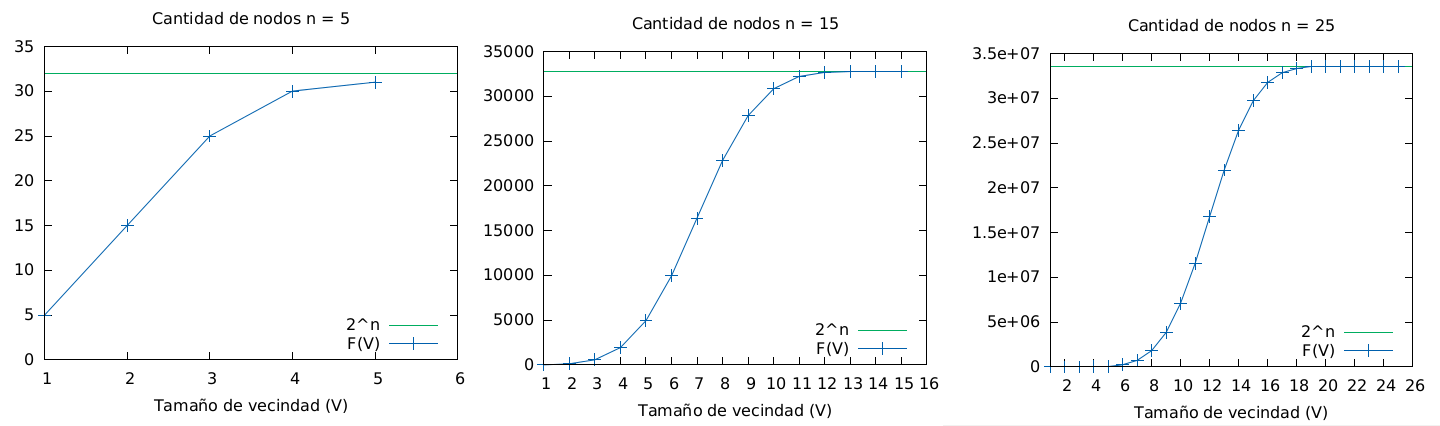
\includegraphics[scale=0.32]{imgs/v.png}
\end{center}

\par{Al incrementar el $n$, son más los valores de $V$ para los cuales $F(V)$
es insignificante frente a la complejidad de $2^n$. Si bien es cierto que $V$
podría tomar valores hasta al rededor de $n/5$ sin alterar la complejidad del
algoritmo, se espera que los valores utilizados no sean mayores a $3$,
incluso para valores de $n$ mucho más grandes. Es por esto que se considerará
la complejidad en función de $V$ con $F(V)$, si bien es cierto que, formalmente,
esta complejidad está acotada superiormente por $2^n$.}\\
 
\par{Finalmente, la complejidad de la implementación de búsqueda local es\\
$(m-f_i) * F(V) * V*\Delta(G) \in$ O($m*2^n*n$). Si bien esta
complejidad parece excesiva para una heurística (de hecho es mayor a la
complejidad de evaluar todas las soluciones), hay dos razones que nos llevan a
pensar que en la práctica se comportará mejor. En primer lugar, deben tomarse
instancias muy específicas (o parámetros muy malos) para que la cantidad de
iteraciones se acerque a $m$. Es esperable que, de haber muchas soluciones
vecinas mejores, se consiga una de frontera varias
veces mayor a la actual y no necesariamente mejorar siempre de a uno, con
lo cual, la cantidad de iteraciones estaría lejos del valor de $m$.}\\

\par{En segundo lugar, la elección del parámetro $V$.
Con un tamaño de vecindad de $V = 1$, la cantidad de vecinos de cada solución es
$F(1) = \binom{n}{1} = n$ la cual es una buena cantidad de vecinos y
resulta en una complejidad de O($m*n*n$). La cantidad de aristas $m$ se puede
acotar por $n^2$ con lo que la complejidad sería $n^2 * n * n \in$
O($n^4$), es decir, es polinomial. Incluso si $V$ fuese 2 o 3 los tiempos
de ejecución tampoco se acercarían a la complejidad del algoritmo exacto.}

\subsection{Comportamiento}

\par{El índice de optimalidad (que tan cercana a la solución óptima es la
solución devuelta) de la heurística de búsqueda local depende mucho del
parámetro $V$, así como de la solución inicial. Si la solución inicial
es una tal que todas sus vecinas son peores (estrictamente) que ella, el
algoritmo no mejorará la solución y devolverá la solución inicial. Como ya se
mencionó, una vecindad muy pequeña tiene más posibilidades de estancarse en
un óptimo local cuando en la misma instancia una vecindad mayor permitiría
alcanzar soluciones mejores.}\\

\par{La única cota inferior a la frontera de la solución devuelta por esta
heurística es la frontera de la solución inicial, la cual puede diferir de la
frontera de la solución óptima tanto como uno quiera. En grafos con grados
pequeños, la heurística tiene mayores posibilidades de encontrar una solución
óptima. De hecho, si se ejecuta el algoritmo con $V$ = $\Delta$($G$) y la
solución inicial igual al conjunto vacío, la vecindad de la solución inicial
en la primera iteración incluirá todas las posibles cliques del grafo, es decir
que en una sola iteración obtendrá la solución óptima. Cuando $\Delta$($G$) es
demasiado grande, no tiene sentido hacer eso, ya que la complejidad superaría
la del algoritmo exacto.}

\subsection{Experimentación}

\subsubsection{Performance}

\par{El archivo $test\_local.cpp$ en la carpeta $codigo/local$ contiene la
implementación del código que mide los tiempos de ejecución de la heurística
de búsqueda local. Se ejecutó este programa con $N$ = 1200, $s$ = 20 y $k$ = 10.
Es decir, para cada $n$ entero múltiplo de 20, entre 20 y 1200, se generaron
10 grafos aleatorios (con la función $generar\_aristas\_aleatorias$). Para cada
instancia generada se corrieron tres versiones de la heurística de búsqueda
local. Con V=1, con V=2 y con V=3. Para las tres, la solución inicial fue la
solución vacía.
En el siguiente gráfico se muestran los resultados obtenidos.}

\begin{center}
\textbf{Gráfico de performance de la heurística de búsqueda local\\ en
función de la cantidad de nodos del grafo}
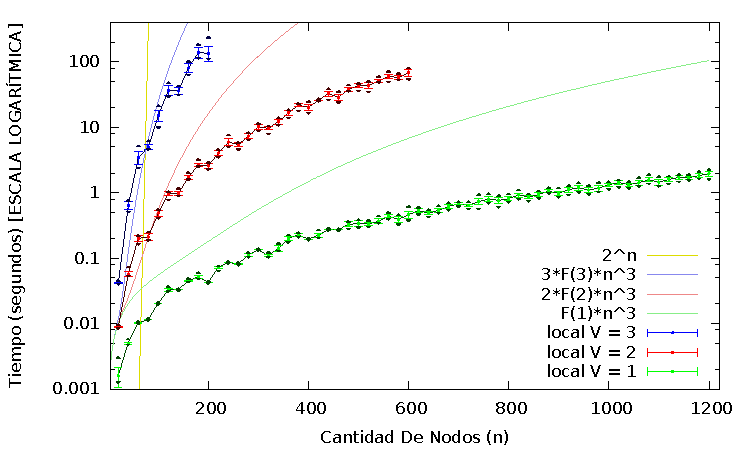
\includegraphics[scale=1.3]{imgs/local_1200_20_10.pdf}
\end{center}

\par{Cada punto $\bullet$ en el gráfico representa el promedio de los tiempos
medidos para cada una de las 10 ejecuciones de una determinada cantidad de nodos
del grafo. El tamaño del segmento vertical sobre cada punto $\bullet$ representa
su varianza asociada. Además, para cada cantidad de nodos $n$ se graficaron la
máxima medición con $\blacktriangle$ y la mínima medición con
$\blacktriangledown$.}\\

\par{La función graficada con una curva amarilla es una función exponencial de
base 2. Al estar utilizando escala logarítmica en el eje de ordenadas, esta curva
se ve como una recta. También se graficaron otras tres funciones para que acoten
superiormente cada una de las heurísticas, basándose en su complejidad estimada
en función de $F(V)$. Como se puede observar, si bien incrementando el $V$ los
tiempos de ejecución de la heurística aumentan considerablemente, están muy
lejos de asemejarse a la curva de la función exponencial\footnote{Para que
las comparaciones tengan sentido, las cuatro funciones graficadas fueron
multiplicadas por las mismas constantes. Es por ello que fue difícil ajustar
las tres cotas superiores a las curvas definidas por las tres heurísticas.},
la cual se ve en el gráfico como una recta casi vertical.}

\subsubsection{Optimalidad}

\par{El archivo $opt\_local.cpp$ en la carpeta $codigo/local$ contiene la
implementación del código que mide el índice de optimalidad de la heurística
de búsqueda local. Se ejecutó este programa con $N$ = 100\footnote{Para el test
de performance ejecutamos instancias de tamaño 1200. Sin embargo, para calcular
la optimalidad de la heurísica también debemos ejecutar el algoritmo exacto
con cada instancia, lo que nos restringe el máximo tamaño de entrada.},
$s$ = 2 y $k$ = 10. Es decir, para cada $n$ entero par entre 2 y 100, se
generaron 10 grafos aleatorios (con la función $generar\_aristas\_aleatorias$).
Para cada instancia generada se corrieron las mismas tres versiones de la
heurística de búsqueda local. Para las tres, la solución inicial fue la
solución vacía. Para que los datos no se amontonen, utlizamos $s$ = 2 en lugar
de\\$s$ = 1.
En el siguiente gráfico se muestran los resultados obtenidos.}

\begin{center}
\textbf{Gráfico de optimalidad de la heurística de búsqueda local\\
en función de la cantidad de nodos del grafo}
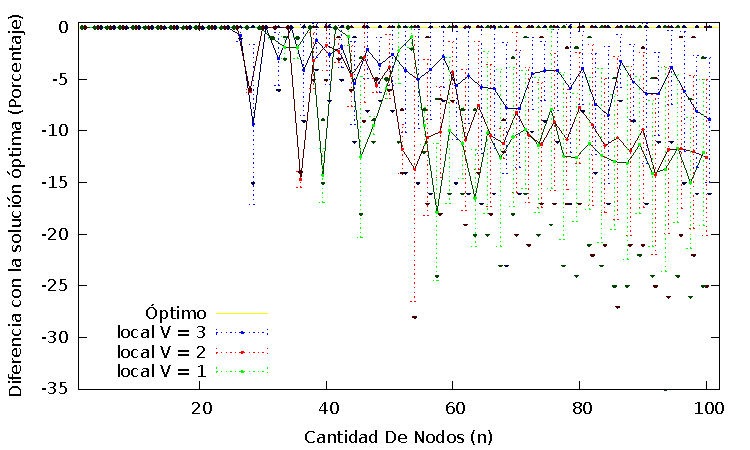
\includegraphics[scale=1.3]{imgs/opt_local_100_2_10.pdf}
\end{center}

\par{Cada punto $\bullet$ en el gráfico representa el promedio del índice de
optimalidad para cada una de las 10 ejecuciones de una determinada cantidad de
nodos del grafo. El tamaño del segmento vertical (en líneas punteadas, también
para que los datos no se amontonen) sobre cada punto $\bullet$
representa su varianza asociada. Además, para cada cantidad de nodos $n$ se
graficaron la máxima medición con $\blacktriangle$ y la mínima medición con
$\blacktriangledown$.}\\

\par{La recta $y=0$ representa la solución óptima, así que cuanto más se
asemeje la curva definida por una heurística a dicha recta, mejor es la
heurística. Como se puede observar, para pequeños valores de $n$ las tres
variantes de la heurística encuentran siempre, o casi siempre, una solución
óptima. Al aumentar la cantidad de nodos, aumentan tanto la diferencia
respecto a la solución óptima, como la varianza asociada.}\\

\par{Como esperábamos, los resultados obtenidos por la variante con $V$=3 son
mejores a los obtenidos por las otras dos variantes. Sin embargo no se ve una
mejora considerable por parte de la variante con $V$=2 respecto a la variante
con $V$=1, de hecho es peor en algunos casos.}\\

\par{Incluso para $n$ mayores, hay instancias para las que las
heurísticas encuentran una solución óptima. Esto se ve en los $\blacktriangle$
que están sobre la curva $y=0$. Aunque para los mismos $n$ hay instancias en
que las soluciones devueltas por las variantes con $V$=1 y $V$=2 difieren en
más del 25\% del óptimo. No es así con la variante con $V$=3, cuyos mínimos en
dichos casos difieren en al rededor del 15\% respecto a la solución óptima y tiene
más casos en los que encuentra una solución óptima, que las otras dos variantes.
Como esperábamos, la varianza en el índice de optimalidad de la heurística
es muy grande debido a que este depende mucho del tipo de grafo que resuelve.
Al incrementar la cantidad de nodos, las curvas definidas por los resultados de
los algoritmos parecen estabilizarse. En promedio la variante con $V$=3 parece
encontrar soluciones que representan entre el 5\% y el 10\% del óptimo, mientras
que las otras dos variantes parecen estabilizarse entre el 10\% y el 15\%.
También parece que ninguna de las tres variantes es peor del 35\%.}
